\documentclass{standalone}
\usepackage{pgfplots}
\usetikzlibrary{arrows.meta}
\pgfplotsset{compat=newest}
\begin{document}
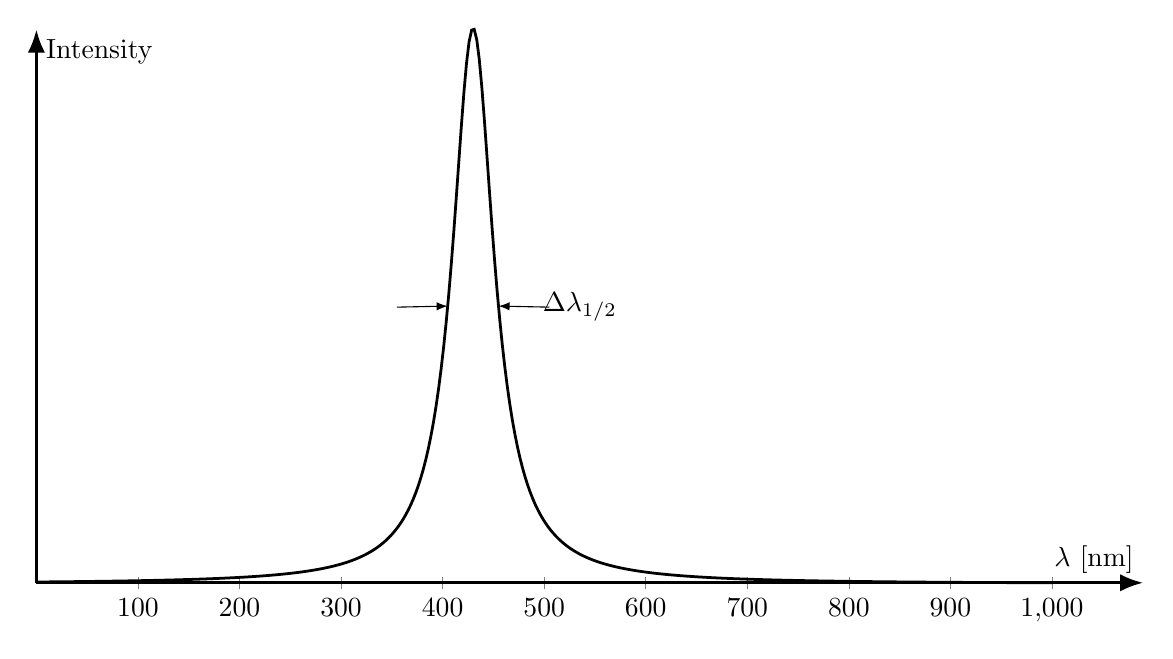
\begin{tikzpicture}
\begin{axis}[
axis lines=center, ytick=\empty,
xlabel={$\lambda$ [nm]},
ylabel={Intensity},
xmin=0,xmax=1090,
xmajorgrids=false,
clip=false,
inner axis line style={-Latex,very thick},
scale only axis=true,
height=200pt,
width=400pt,
]
\addplot[line width=1pt,samples=400,domain=0:1000]
{100^2/((x-430)^2+25^2)};
\draw[latex-] (axis cs:455,8) -- node[right]{$\ \Delta \lambda_{1/2}$} +(50,0);
\draw[latex-] (axis cs:405,8) -- +(-50,0);
\end{axis}
\end{tikzpicture}
\end{document}